\section{Labeling Tool}\label{sec:labeling-tool}

Um die Erstellung und Verwaltung von gelabelten \ac{BPMN}-Prozessmodellen zu erleichtern, wurde eine Webapp entwickelt. Mit dieser können \ac{BPMN}-Testfälle erstellt, bearbeitet und Aktivitäten mit Labeln versehen werden. Wichtige Funktionen des Labeling-Tools sind dabei: (1) das Anlegen und Verwalten von Datensätzen, (2) die Erstellung beliebig vieler Testfälle pro Datensatz, (3) die direkte Bearbeitung von \ac{BPMN}-Modellen im Browser mittels BPMN.io \cite{bpmnio}, (4) ein Labeling-Modus, in dem Aktivitäten als \ac{DSGVO}-kritisch markiert und optional mit einer Begründung versehen werden können, sowie (5) die persistente Speicherung der annotierten Testfälle in einer Datenbank zur späteren Nutzung im Evaluationsframework (siehe Kapitel~\ref{ch:evaluationsframework}).

Abbildung \ref{fig:labeling-editor} zeigt den Labeling-Editor im Labeling-Modus. Die in der Abbildung nummerierten Bereiche strukturieren die Oberfläche und das Zusammenspiel der Funktionen:

\begin{figure}{h}
    \centering
    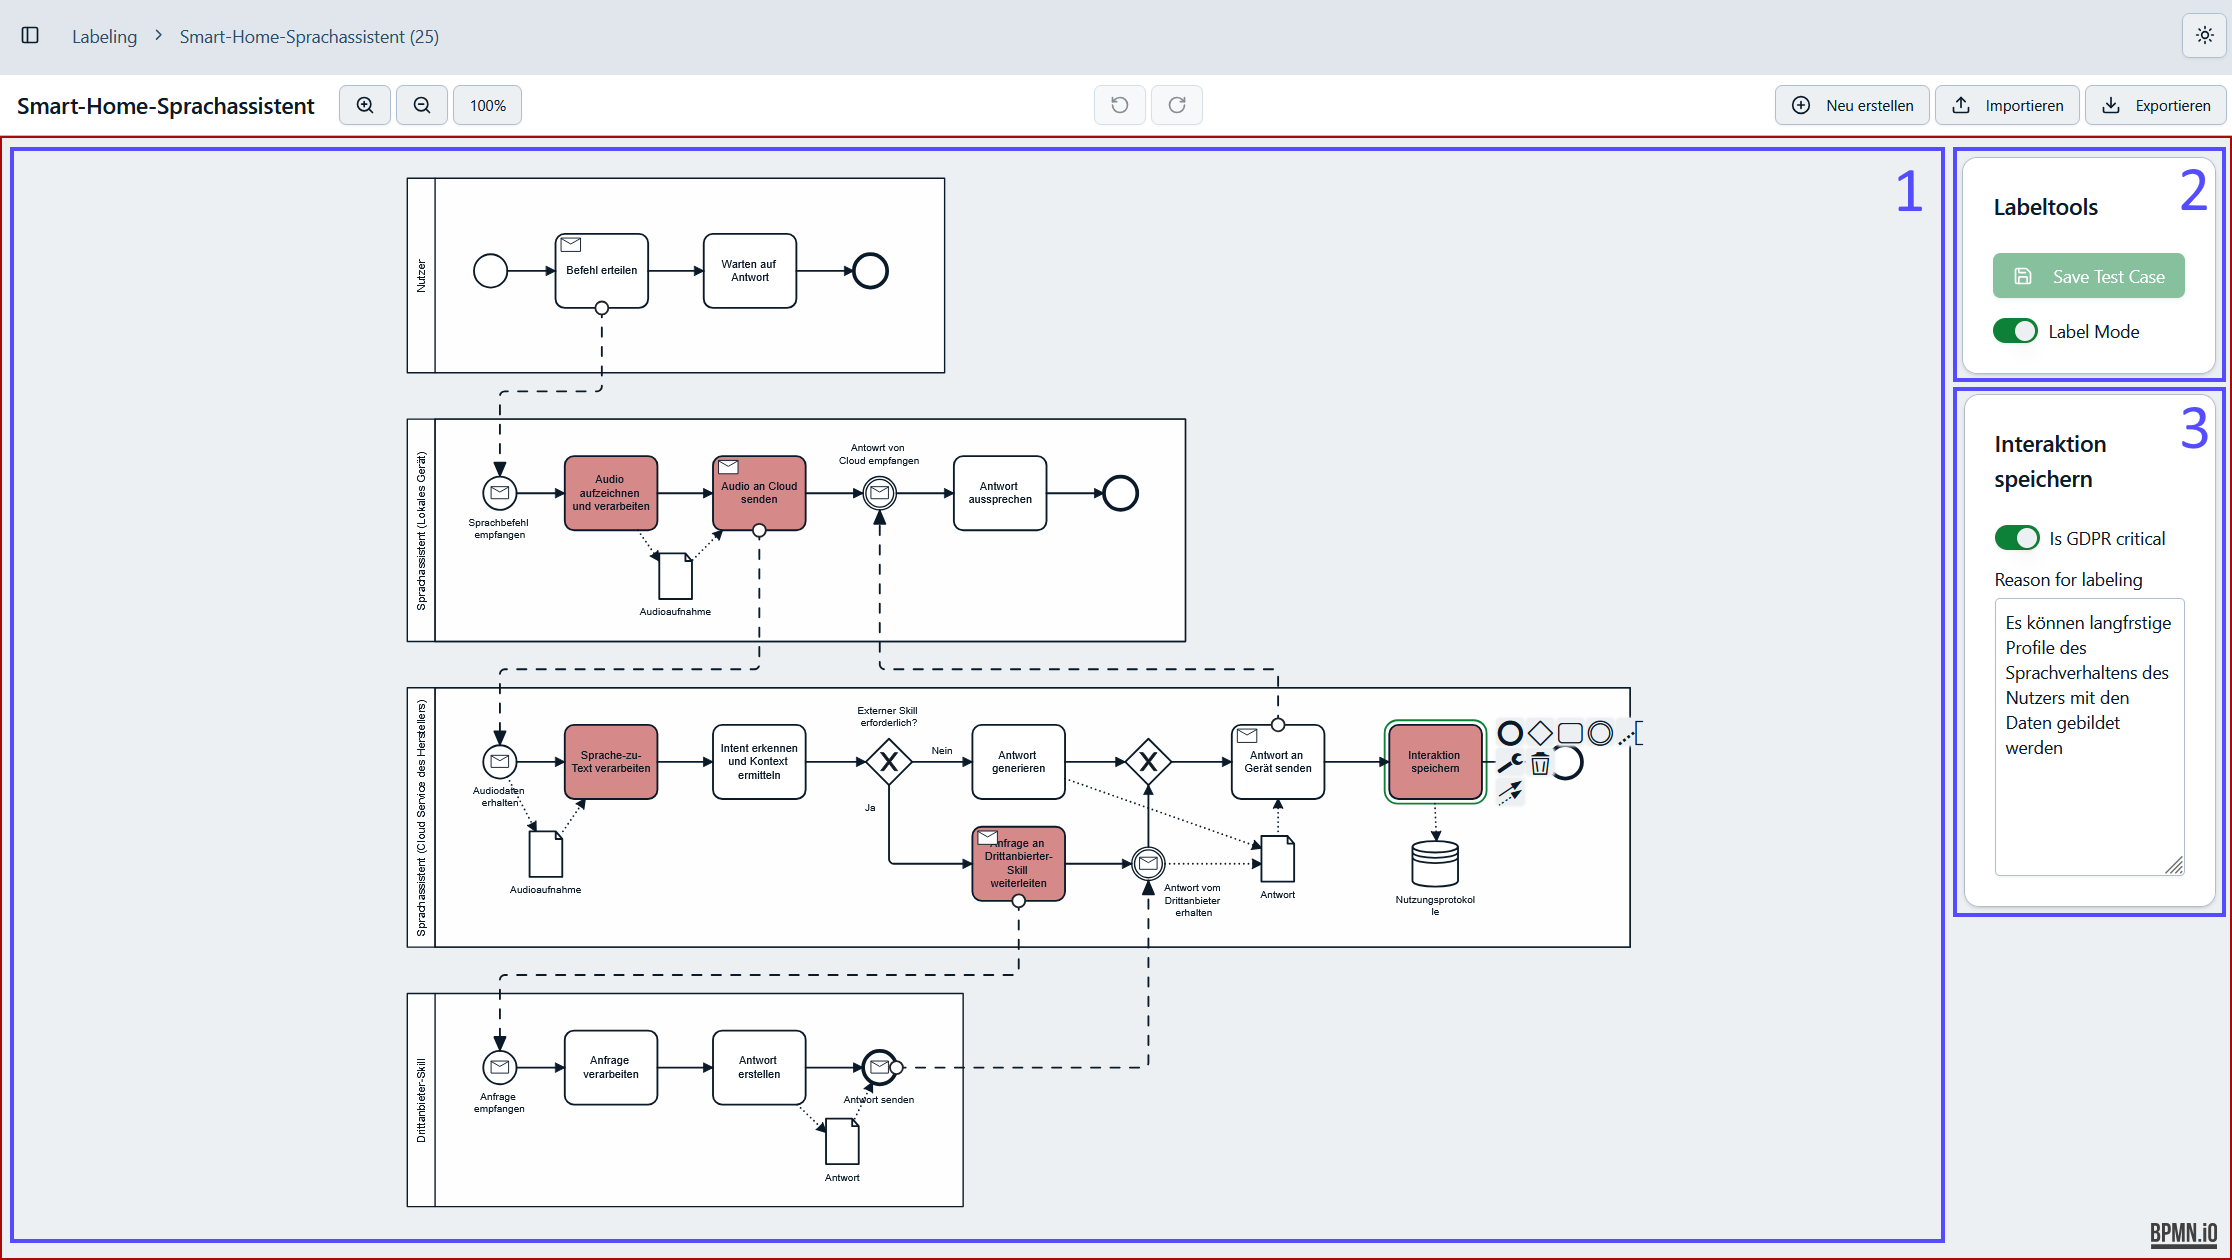
\includegraphics[width=\textwidth]{images/labeling/labeling-editor-annotated}
    \caption{Labeling-Editor im Labeling-Modus mit exemplarischem Modell.}
    \label{fig:labeling-editor}
\end{figure}

\begin{enumerate}
    \item \textbf{BPMN-Editor} (linke Hauptfläche): Hier werden Prozessmodelle erstellt, importiert, bearbeitet und angezeigt. Im Labeling-Modus ist die Modellierung bewusst gesperrt. Die Elemente können dann nur ausgewählt werden, um sie zu labeln. Als kritisch gelabelte Aktivitäten werden im Modell farblich hervorgehoben und sind damit sofort visuell erkennbar.
    \item \textbf{Label-Tools} (rechte Seitenleiste oben): Über dieses Panel wird zwischen Editier- und Labeling-Modus gewechselt und ein Testfall gespeichert.
    \item \textbf{Label-Panel der Aktivität} (rechte Seitenleiste unten): Ist eine Aktivität ausgewählt, kann sie hier als \enquote{DSGVO-kritisch} markiert werden. Zusätzlich lässt sich optional eine natürlichsprachige Begründung hinterlegen. Diese Begründung dient ausschließlich der Dokumentation und Nachvollziehbarkeit und wird nicht in der Evaluierung berücksichtigt.
\end{enumerate}

In der Übersicht der Datensätze aus Abbildung \ref{fig:labeling-datasets} sind alle angelegten Datensätze und zugehörigen Testfälle aufgelistet. Von hier aus können neue Datensätze und Testfälle erstellt sowie bestehende bearbeitet werden.

\begin{figure}[h]
    \centering
    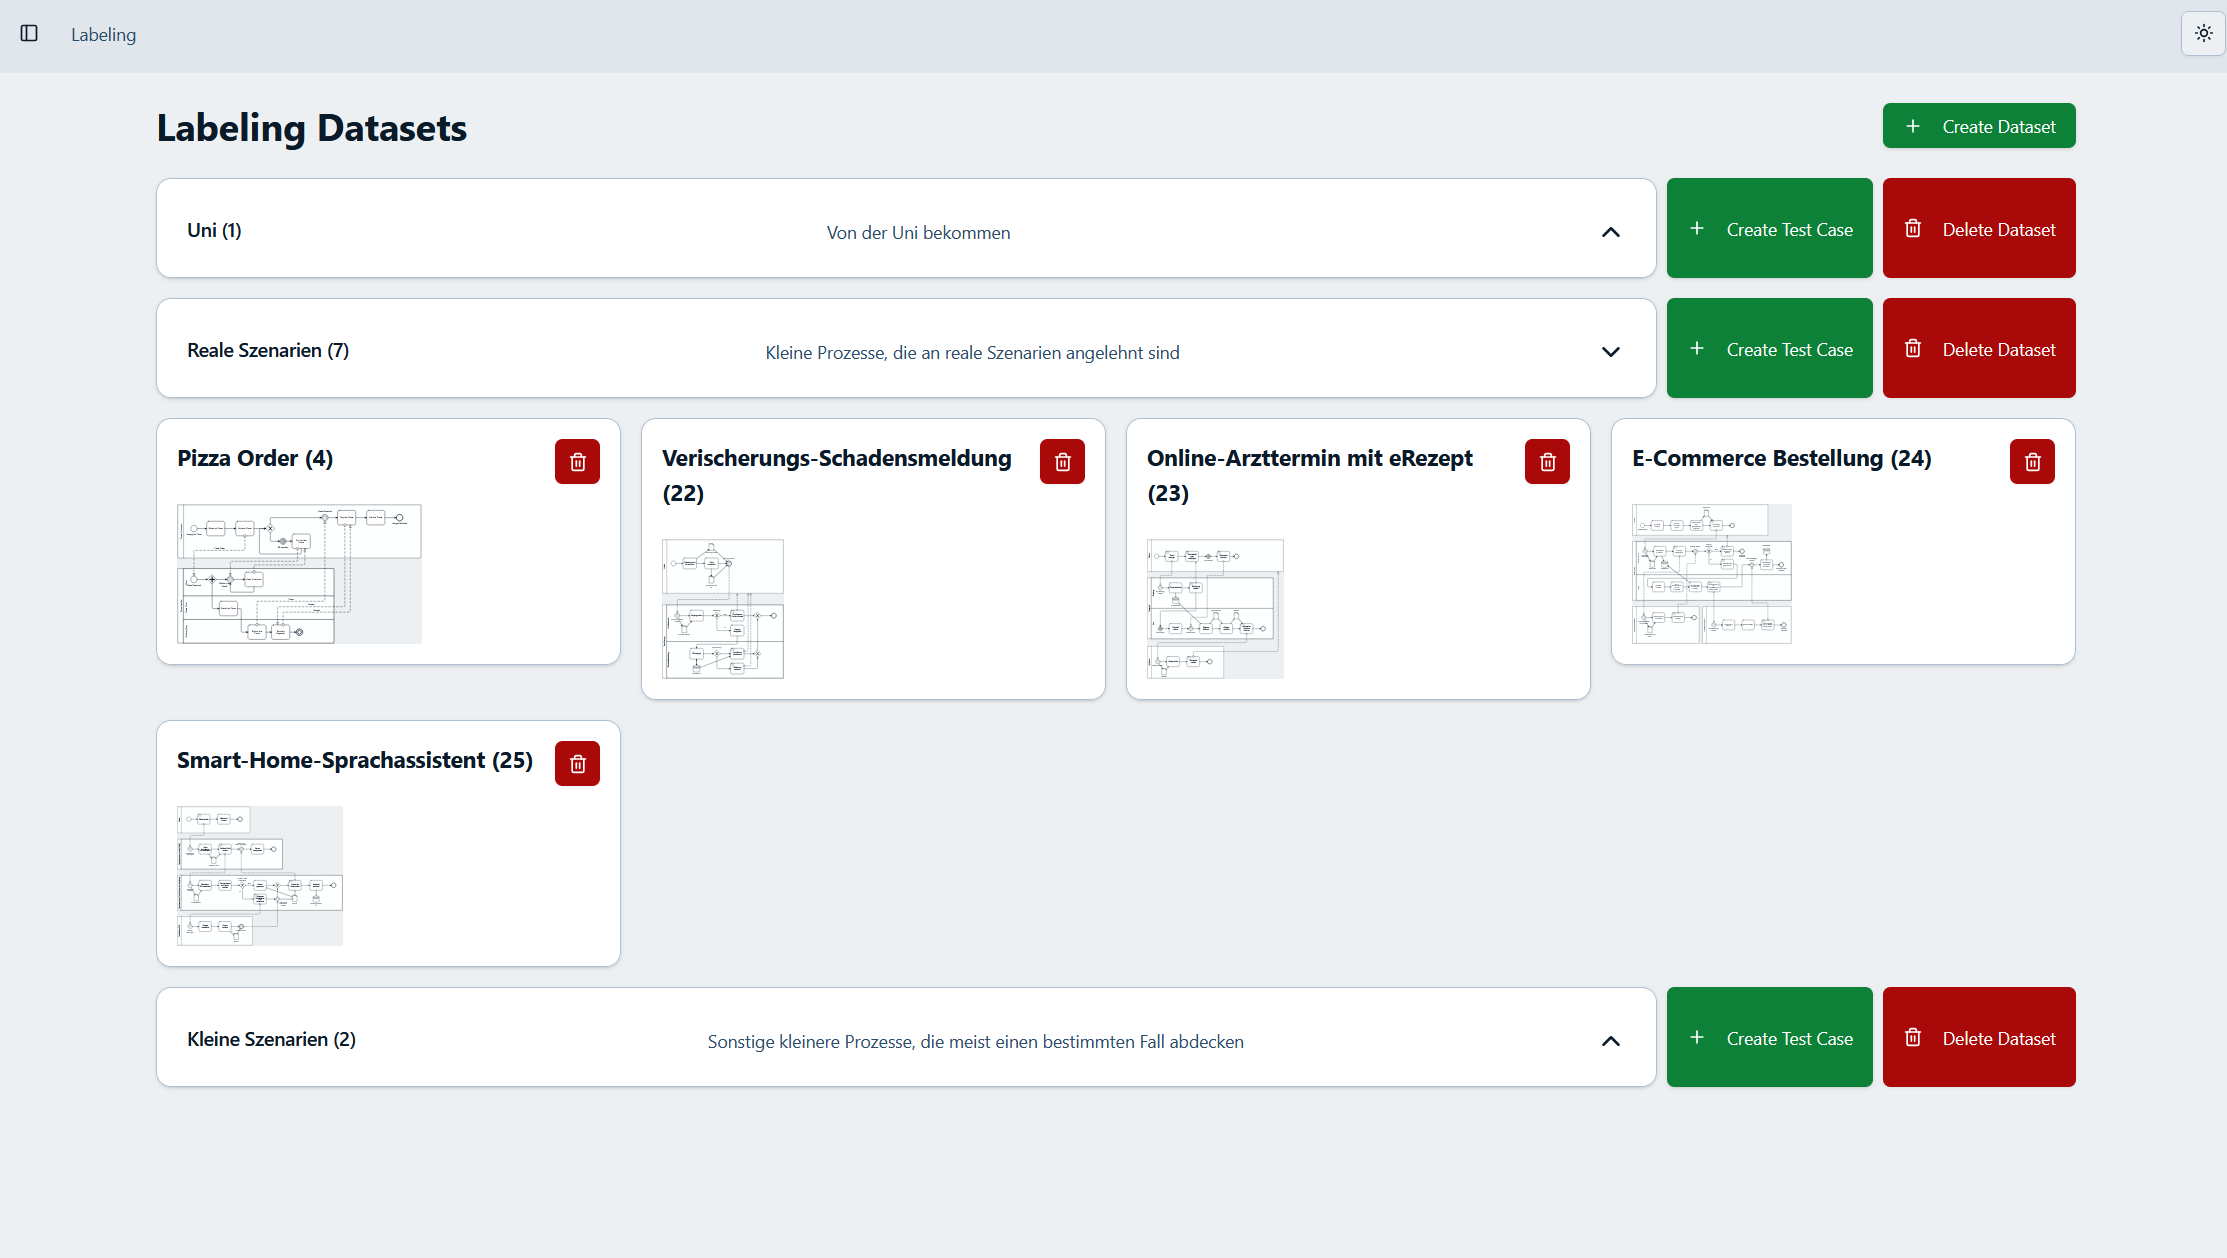
\includegraphics[width=\textwidth]{images/labeling/labeling-datasets}
    \caption{Übersicht der Datensätze im Labeling-Tool.}
    \label{fig:labeling-datasets}
\end{figure}